\documentclass[aspectratio=169,10pt]{beamer}
\usetheme{default}
\usefonttheme{professionalfonts}

\usepackage[OT1]{fontenc}
\usepackage[utf8]{inputenc}
\usepackage[protrusion=true,expansion=true]{microtype}
\renewcommand{\familydefault}{\sfdefault}
\usepackage{tikz}
\usepackage{booktabs}
\usepackage{array}
\usetikzlibrary{arrows.meta,positioning,calc,fit,backgrounds,shapes.geometric,decorations.pathreplacing}

\definecolor{DeepNavy}{RGB}{8,29,57}
\definecolor{Blue}{RGB}{36,99,180}
\definecolor{Cyan}{RGB}{30,163,195}
\definecolor{GraphPurple}{RGB}{103,80,164}
\definecolor{Amber}{RGB}{204,143,40}
\definecolor{Red}{RGB}{178,55,67}
\definecolor{Teal}{RGB}{31,137,145}
\definecolor{Green}{RGB}{70,138,86}
\definecolor{Slate}{RGB}{88,98,112}
\definecolor{SoftBlue}{RGB}{224,236,250}
\definecolor{SoftCyan}{RGB}{220,244,248}
\definecolor{SoftPurple}{RGB}{235,229,247}
\definecolor{SoftAmber}{RGB}{253,240,214}
\definecolor{SoftRed}{RGB}{250,226,229}
\definecolor{SoftTeal}{RGB}{221,242,241}
\definecolor{SoftGreen}{RGB}{226,242,230}
\definecolor{SoftSlate}{RGB}{235,238,242}
\definecolor{Canvas}{RGB}{247,250,253}

\setbeamercolor{normal text}{fg=DeepNavy,bg=white}
\setbeamercolor{frametitle}{fg=DeepNavy,bg=white}
\setbeamercolor{title}{fg=white,bg=DeepNavy}
\setbeamercolor{structure}{fg=Blue}
\setbeamertemplate{navigation symbols}{}
\setbeamertemplate{footline}{%
  \hfill\usebeamerfont{page number in head/foot}\insertframenumber/\inserttotalframenumber\hspace{0.45cm}\vspace{0.18cm}}
\setbeamersize{text margin left=9mm,text margin right=9mm}
\setbeamerfont{title}{series=\bfseries,size=\LARGE}
\setbeamerfont{subtitle}{size=\large}
\setbeamerfont{frametitle}{series=\bfseries,size=\Large}
\setbeamerfont{normal text}{size=\normalsize}

\tikzset{
  >=Latex,
  box/.style={draw=DeepNavy,thick,rounded corners=4pt,fill=white,align=center,text=DeepNavy,font=\small,minimum height=.86cm,inner xsep=7pt,inner ysep=5pt},
  service/.style={box,draw=Blue,fill=SoftBlue},
  transform/.style={box,draw=Teal,fill=SoftTeal},
  graph/.style={box,draw=GraphPurple,fill=SoftPurple},
  warn/.style={box,draw=Amber,fill=SoftAmber},
  err/.style={box,draw=Red,fill=SoftRed},
  ok/.style={box,draw=Green,fill=SoftGreen},
  storage/.style={cylinder,shape border rotate=90,aspect=.25,draw=Slate,thick,fill=SoftSlate,align=center,text=DeepNavy,font=\small,minimum width=1.55cm,minimum height=1.12cm},
  future/.style={box,draw=Slate,dash pattern=on 4pt off 2pt,fill=white,text=Slate},
  note/.style={font=\small,text=Slate,align=center},
  label/.style={font=\bfseries\small,text=DeepNavy,align=center},
  nodeInfo/.style={circle,draw=Blue,very thick,fill=SoftBlue,text=DeepNavy,font=\bfseries\small,minimum size=.72cm,inner sep=1pt},
  nodeWarn/.style={circle,draw=Amber,very thick,fill=SoftAmber,text=DeepNavy,font=\bfseries\small,minimum size=.72cm,inner sep=1pt},
  nodeErr/.style={circle,draw=Red,very thick,fill=SoftRed,text=DeepNavy,font=\bfseries\small,minimum size=.78cm,inner sep=1pt},
  nodeDbg/.style={circle,draw=Slate,very thick,fill=SoftSlate,text=DeepNavy,font=\bfseries\small,minimum size=.70cm,inner sep=1pt},
  outnode/.style={circle,draw=Slate,thick,fill=SoftSlate,text=Slate,font=\small,minimum size=.64cm,inner sep=1pt},
  flow/.style={-{Latex[length=3mm,width=2.2mm]},line width=1.25pt,draw=Cyan,shorten >=3pt,shorten <=3pt},
  data/.style={-{Latex[length=3mm,width=2.2mm]},line width=1.2pt,draw=Slate,shorten >=3pt,shorten <=3pt},
  req/.style={-{Latex[length=3mm,width=2.2mm]},line width=1.25pt,draw=GraphPurple,shorten >=4pt,shorten <=4pt},
  res/.style={-{Latex[length=3mm,width=2.2mm]},line width=1.25pt,dashed,draw=Teal,shorten >=4pt,shorten <=4pt},
  control/.style={-{Latex[length=2.7mm,width=2mm]},line width=1.1pt,dashed,draw=Amber,shorten >=3pt,shorten <=3pt},
  futureline/.style={-{Latex[length=2.7mm,width=2mm]},line width=1.1pt,dash pattern=on 4pt off 2pt,draw=Slate,shorten >=3pt,shorten <=3pt}
}

\newcommand{\progress}[1]{%
  \begin{tikzpicture}[remember picture,overlay]
    \node[anchor=north west,inner sep=0pt] at ($(current page.north west)+(0.52,-0.08)$) {%
      \begin{tikzpicture}[x=1cm,y=1cm]
        \draw[Red,line width=1.3pt] (0,0)--(1.85,0);
        \draw[Blue,line width=1.3pt] (1.85,0)--(3.7,0);
        \draw[GraphPurple,line width=1.3pt] (3.7,0)--(5.55,0);
        \draw[Amber,line width=1.3pt] (5.55,0)--(7.4,0);
        \draw[Teal,line width=1.3pt] (7.4,0)--(9.25,0);
        \draw[Green,line width=1.3pt] (9.25,0)--(11.1,0);
      \end{tikzpicture}};
  \end{tikzpicture}}

\title{OpenStack RCA Copilot}
\subtitle{Converting noisy OpenStack logs into structured, bounded, explainable investigation evidence}
\author{Technical Research / Demo Presentation}
\date{\today}

\begin{document}

\begin{frame}[plain]
\begin{tikzpicture}[remember picture,overlay]
  \fill[DeepNavy] (current page.south west) rectangle (current page.north east);
  \node[align=left,text=white,font=\bfseries\LARGE,text width=10.8cm] at ($(current page.center)+(-.55,1.25)$) {OpenStack RCA Copilot};
  \node[align=left,text=SoftCyan,font=\large,text width=11.2cm] at ($(current page.center)+(-.35,.28)$) {Noisy cloud logs become structured, bounded, explainable investigation evidence.};
  \node[align=center,text=white,font=\large] at ($(current page.center)+(0,-1.35)$) {Logs $\rightarrow$ Events $\rightarrow$ Graph $\rightarrow$ Incident Evidence $\rightarrow$ Horizon $\rightarrow$ Grounded AI};
  \draw[Cyan,line width=1.6pt] ($(current page.center)+(-5.6,-.55)$) -- ($(current page.center)+(5.6,-.55)$);
\end{tikzpicture}
\end{frame}

\begin{frame}{1. Hook: Evidence Overload}
\progress{Red}
\centering
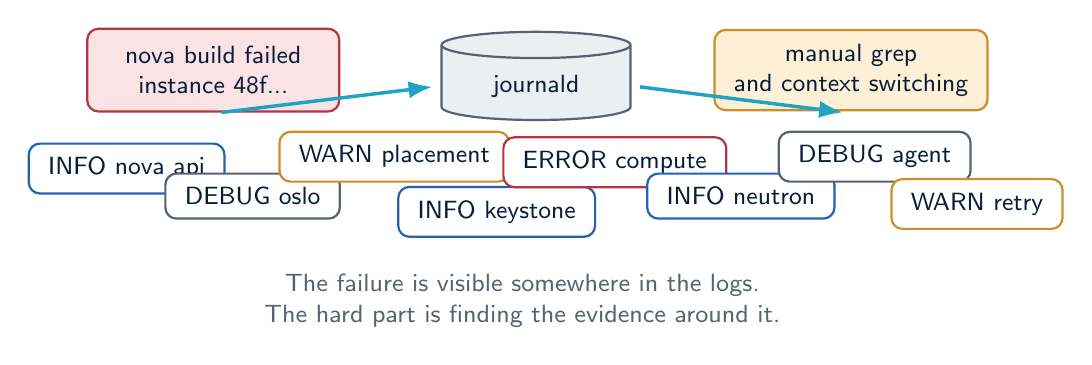
\begin{tikzpicture}[x=1cm,y=1cm]
  \node[err,minimum width=3.2cm,minimum height=1.05cm] at (2.1,3.65) {nova build failed\\instance 48f...};
  \node[storage,minimum width=2.4cm] (j) at (6.2,3.45) {journald};
  \node[warn,minimum width=3.0cm] at (10.2,3.65) {manual grep\\and context switching};
  \foreach \x/\y/\txt/\col in {
    1.0/2.40/INFO nova api/Blue,2.6/2.05/DEBUG oslo/Slate,4.4/2.55/WARN placement/Amber,
    5.7/1.85/INFO keystone/Blue,7.2/2.48/ERROR compute/Red,8.8/2.05/INFO neutron/Blue,
    10.5/2.55/DEBUG agent/Slate,11.8/1.95/WARN retry/Amber}{
    \node[box,draw=\col,fill=white,minimum width=1.45cm,minimum height=.56cm,font=\small] at (\x,\y) {\txt};
  }
  \draw[flow] (2.1,3.1)--(j.west);
  \draw[flow] (j.east)--(10.2,3.1);
  \node[note,text width=10.5cm] at (6,.72) {The failure is visible somewhere in the logs. The hard part is finding the evidence around it.};
\end{tikzpicture}
\end{frame}

\begin{frame}{2. Problem: Logs Are Noisy, Distributed, and Hard to Connect}
\progress{Red}
\centering
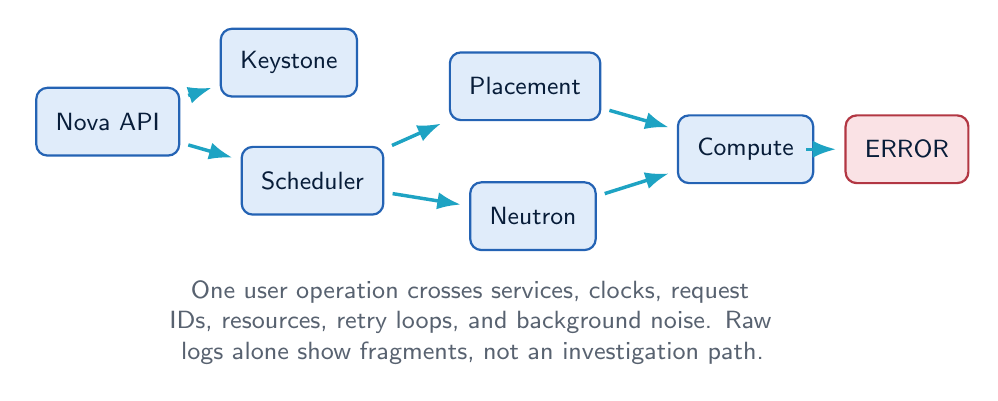
\begin{tikzpicture}[x=1cm,y=1cm]
  \node[service] (api) at (1.4,3.25) {Nova API};
  \node[service] (key) at (3.7,4.0) {Keystone};
  \node[service] (sch) at (4.0,2.5) {Scheduler};
  \node[service] (pl) at (6.7,3.7) {Placement};
  \node[service] (neu) at (6.8,2.05) {Neutron};
  \node[service] (cmp) at (9.5,2.9) {Compute};
  \node[err] (e) at (11.55,2.9) {ERROR};
  \draw[flow] (api)--(key);
  \draw[flow] (api)--(sch);
  \draw[flow] (sch)--(pl);
  \draw[flow] (sch)--(neu);
  \draw[flow] (pl)--(cmp);
  \draw[flow] (neu)--(cmp);
  \draw[flow] (cmp)--(e);
  \node[note,text width=11cm] at (6,.7) {One user operation crosses services, clocks, request IDs, resources, retry loops, and background noise. Raw logs alone show fragments, not an investigation path.};
\end{tikzpicture}
\end{frame}

\begin{frame}{3. Insight: Every Log Can Become a Structured Event}
\progress{Blue}
\centering
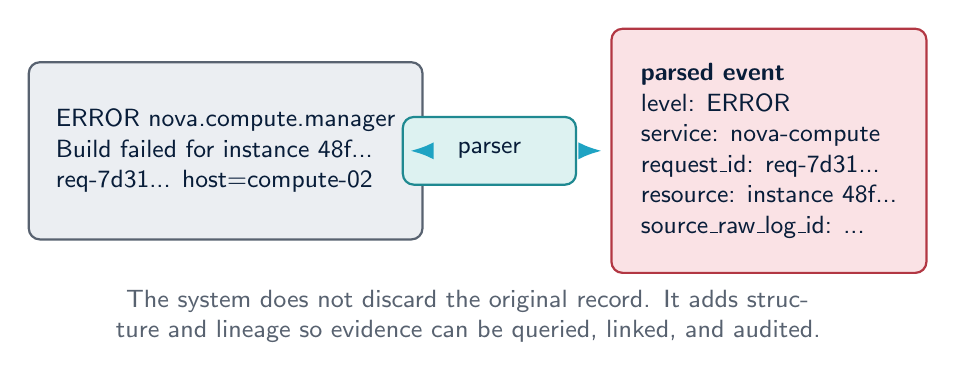
\begin{tikzpicture}[x=1cm,y=1cm]
  \node[box,draw=Slate,fill=SoftSlate,minimum width=5.0cm,minimum height=2.25cm,align=left] (raw) at (2.95,2.75) {
    ERROR nova.compute.manager\\
    Build failed for instance 48f...\\
    req-7d31... host=compute-02};
  \node[transform,minimum width=2.2cm] (parser) at (6.3,2.75) {parser};
  \node[box,draw=Red,fill=SoftRed,minimum width=4.0cm,minimum height=3.1cm,align=left] (event) at (9.85,2.75) {
    \textbf{parsed event}\\
    level: ERROR\\
    service: nova-compute\\
    request\_id: req-7d31...\\
    resource: instance 48f...\\
    source\_raw\_log\_id: ...};
  \draw[flow] (raw.east)--(parser.west);
  \draw[flow] (parser.east)--(event.west);
  \node[note,text width=10.4cm] at (6,.65) {The system does not discard the original record. It adds structure and lineage so evidence can be queried, linked, and audited.};
\end{tikzpicture}
\end{frame}

\begin{frame}{4. Pipeline Overview: The Mental Model}
\progress{Blue}
\centering
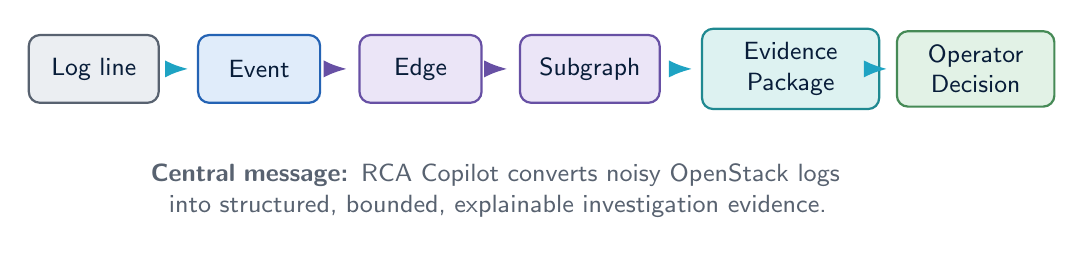
\begin{tikzpicture}[x=1cm,y=1cm]
  \node[box,draw=Slate,fill=SoftSlate,minimum width=1.65cm] (log) at (.9,2.8) {Log line};
  \node[service,minimum width=1.55cm] (event) at (3.0,2.8) {Event};
  \node[graph,minimum width=1.55cm] (edge) at (5.05,2.8) {Edge};
  \node[graph,minimum width=1.75cm] (sub) at (7.2,2.8) {Subgraph};
  \node[transform,minimum width=2.25cm] (pkg) at (9.75,2.8) {Evidence\\Package};
  \node[ok,minimum width=2.0cm] (op) at (12.1,2.8) {Operator\\Decision};
  \draw[flow] (log)--(event);
  \draw[req] (event)--(edge);
  \draw[req] (edge)--(sub);
  \draw[flow] (sub)--(pkg);
  \draw[flow] (pkg)--(op);
  \node[note,text width=11cm] at (6,1.25) {\textbf{Central message:} RCA Copilot converts noisy OpenStack logs into structured, bounded, explainable investigation evidence.};
\end{tikzpicture}
\end{frame}

\begin{frame}{5. Current Implementation Status}
\progress{Blue}
\centering
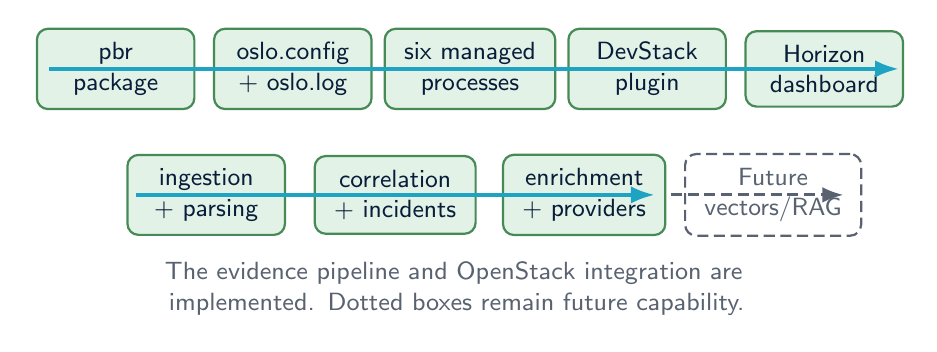
\begin{tikzpicture}[x=1cm,y=1cm]
  \node[ok,minimum width=2.0cm] at (1.7,3.35) {pbr\\package};
  \node[ok,minimum width=2.0cm] at (3.95,3.35) {oslo.config\\+ oslo.log};
  \node[ok,minimum width=2.0cm] at (6.2,3.35) {six managed\\processes};
  \node[ok,minimum width=2.0cm] at (8.45,3.35) {DevStack\\plugin};
  \node[ok,minimum width=2.0cm] at (10.7,3.35) {Horizon\\dashboard};
  \node[ok,minimum width=2.0cm] at (2.85,1.75) {ingestion\\+ parsing};
  \node[ok,minimum width=2.0cm] at (5.25,1.75) {correlation\\+ incidents};
  \node[ok,minimum width=2.0cm] at (7.65,1.75) {enrichment\\+ providers};
  \node[future,minimum width=2.0cm] at (10.05,1.75) {Future\\vectors/RAG};
  \draw[flow] (.75,3.35)--(11.75,3.35);
  \draw[flow] (1.85,1.75)--(8.65,1.75);
  \draw[futureline] (8.65,1.75)--(11.05,1.75);
  \node[note,text width=10.6cm] at (6,.56) {The evidence pipeline and OpenStack integration are implemented. Dotted boxes remain future capability.};
\end{tikzpicture}
\end{frame}

\begin{frame}{6. Ingestion: journald to MongoDB}
\progress{Blue}
\centering
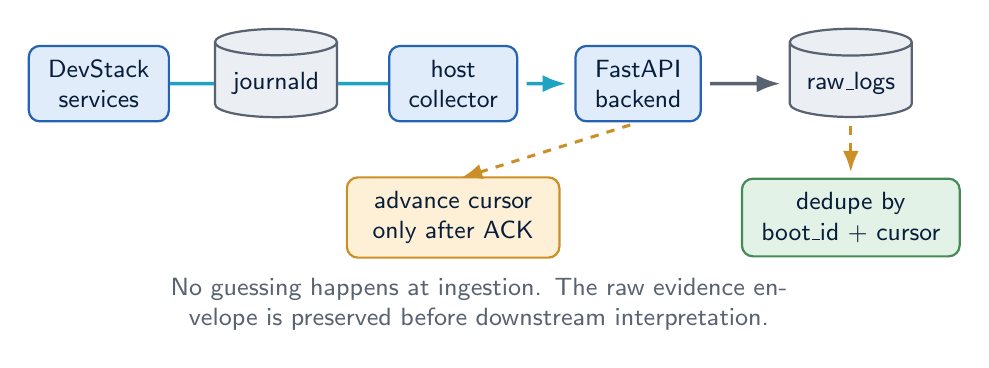
\begin{tikzpicture}[x=1cm,y=1cm]
  \node[service] (dev) at (1.2,3.35) {DevStack\\services};
  \node[storage] (j) at (3.45,3.35) {journald};
  \node[service] (col) at (5.7,3.35) {host\\collector};
  \node[service] (api) at (8.05,3.35) {FastAPI\\backend};
  \node[storage] (raw) at (10.75,3.35) {raw\_logs};
  \node[warn,minimum width=2.7cm] at (5.7,1.65) {advance cursor\\only after ACK};
  \node[ok,minimum width=2.7cm] at (10.75,1.65) {dedupe by\\boot\_id + cursor};
  \draw[flow] (dev)--(j)--(col)--(api);
  \draw[data] (api)--(raw);
  \draw[control] (api.south)--(5.7,2.12);
  \draw[control] (raw.south)--(10.75,2.12);
  \node[note,text width=10.5cm] at (6,.55) {No guessing happens at ingestion. The raw evidence envelope is preserved before downstream interpretation.};
\end{tikzpicture}
\end{frame}

\begin{frame}{7. Parsing: Raw Records to Structured Events}
\progress{Blue}
\centering
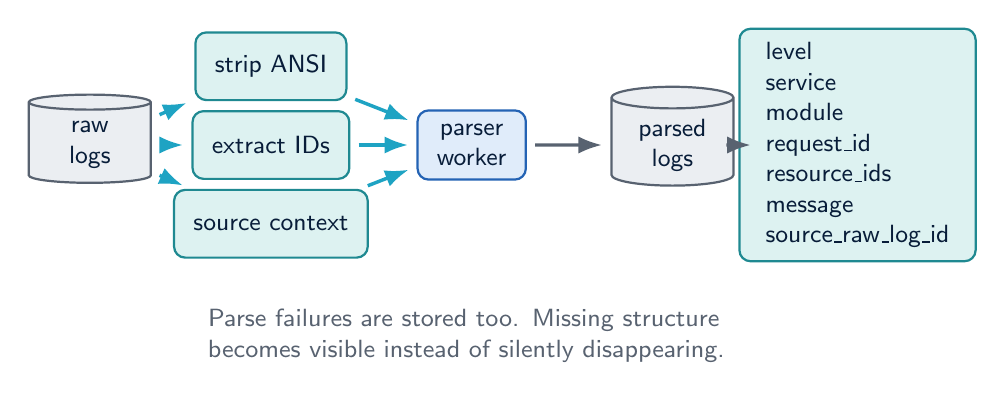
\begin{tikzpicture}[x=1cm,y=1cm]
  \node[storage] (raw) at (1.25,3.0) {raw\\logs};
  \node[transform] (ansi) at (3.55,4.0) {strip ANSI};
  \node[transform] (ids) at (3.55,3.0) {extract IDs};
  \node[transform] (src) at (3.55,2.0) {source context};
  \node[service] (parser) at (6.1,3.0) {parser\\worker};
  \node[storage] (parsed) at (8.65,3.0) {parsed\\logs};
  \node[box,draw=Teal,fill=SoftTeal,minimum width=3.0cm,minimum height=2.9cm,align=left] at (11.0,3.0) {
    level\\service\\module\\request\_id\\resource\_ids\\message\\source\_raw\_log\_id};
  \foreach \n in {ansi,ids,src}{\draw[flow] (raw)--(\n); \draw[flow] (\n)--(parser);}
  \draw[data] (parser)--(parsed);
  \draw[data] (parsed)--(9.75,3.0);
  \node[note,text width=10.4cm] at (6,.58) {Parse failures are stored too. Missing structure becomes visible instead of silently disappearing.};
\end{tikzpicture}
\end{frame}

\begin{frame}{8. Correlation Graph: Request and Resource Links}
\progress{GraphPurple}
\centering
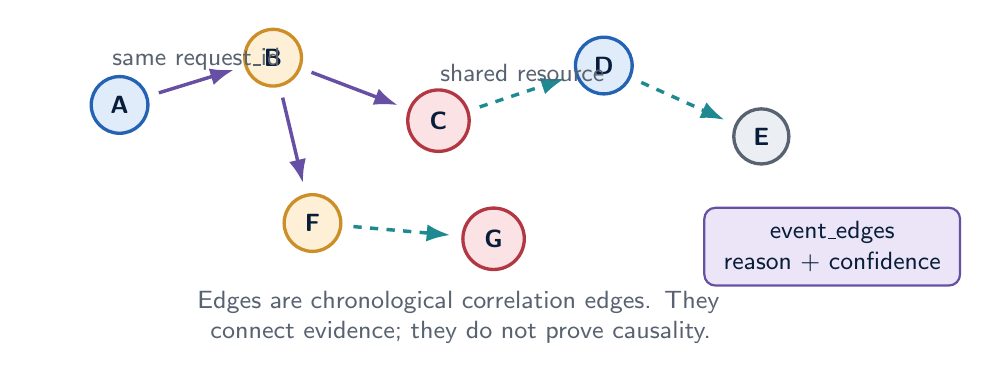
\begin{tikzpicture}[x=1cm,y=1cm]
  \node[nodeInfo] (a) at (1.7,3.25) {A};
  \node[nodeWarn] (b) at (3.65,3.85) {B};
  \node[nodeErr] (c) at (5.75,3.05) {C};
  \node[nodeInfo] (d) at (7.85,3.75) {D};
  \node[nodeDbg] (e) at (9.85,2.85) {E};
  \node[nodeWarn] (f) at (4.15,1.75) {F};
  \node[nodeErr] (g) at (6.45,1.55) {G};
  \draw[req] (a)--node[above,note]{same request\_id}(b);
  \draw[req] (b)--(c);
  \draw[res] (c)--node[above,note]{shared resource}(d);
  \draw[res] (d)--(e);
  \draw[req] (b)--(f);
  \draw[res] (f)--(g);
  \node[graph,minimum width=3.0cm] at (10.75,1.45) {event\_edges\\reason + confidence};
  \node[note,text width=10.7cm] at (6,.55) {Edges are chronological correlation edges. They connect evidence; they do not prove causality.};
\end{tikzpicture}
\end{frame}

\begin{frame}{9. Graph Safety: Why the Graph Does Not Explode}
\progress{GraphPurple}
\centering
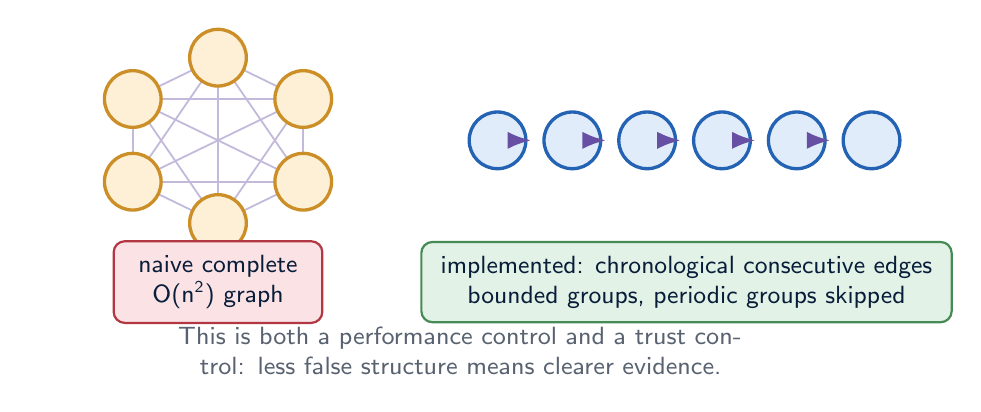
\begin{tikzpicture}[x=1cm,y=1cm]
  \foreach \i/\ang in {1/90,2/30,3/-30,4/-90,5/-150,6/150}{
    \coordinate (p\i) at ({2.95+1.25*cos(\ang)},{3.15+1.05*sin(\ang)});
  }
  \begin{scope}[on background layer]
    \foreach \i in {1,...,5}{\pgfmathtruncatemacro{\s}{\i+1}\foreach \j in {\s,...,6}{\draw[GraphPurple!40,line width=.65pt,shorten >=7pt,shorten <=7pt] (p\i)--(p\j);}}
  \end{scope}
  \foreach \i in {1,...,6}{\node[nodeWarn] at (p\i) {};}
  \node[err,minimum width=2.65cm] at (2.95,1.35) {naive complete\\O(n\textsuperscript{2}) graph};
  \foreach \i/\x in {1/6.5,2/7.45,3/8.40,4/9.35,5/10.30,6/11.25}{\node[nodeInfo] (c\i) at (\x,3.15) {};}
  \foreach \i/\j in {1/2,2/3,3/4,4/5,5/6}{\draw[req] (c\i)--(c\j);}
  \node[ok,minimum width=4.5cm] at (8.9,1.35) {implemented: chronological consecutive edges\\bounded groups, periodic groups skipped};
  \node[note,text width=10.7cm] at (6,.48) {This is both a performance control and a trust control: less false structure means clearer evidence.};
\end{tikzpicture}
\end{frame}

\begin{frame}{10. Incident Construction: Seed Event to Bounded Subgraph}
\progress{Amber}
\centering
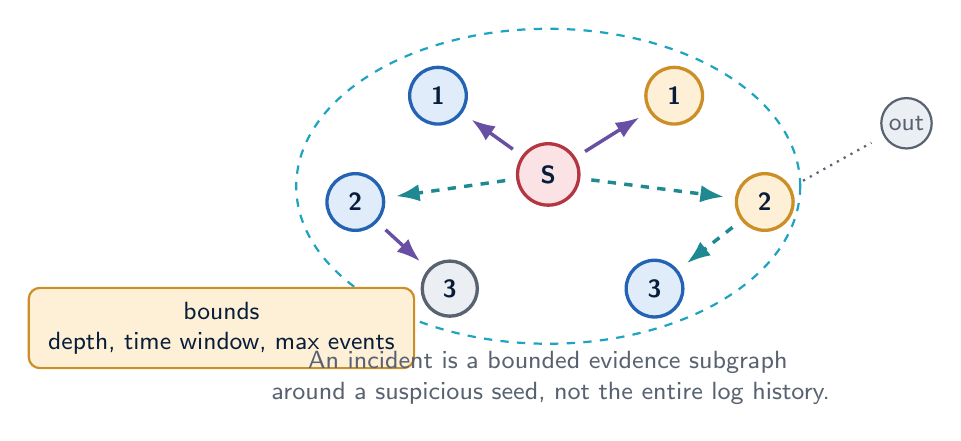
\begin{tikzpicture}[x=1cm,y=1cm]
  \node[nodeErr] (s) at (6,3.0) {S};
  \node[nodeInfo] (a) at (4.6,4.0) {1};
  \node[nodeWarn] (b) at (7.6,4.0) {1};
  \node[nodeInfo] (c) at (3.55,2.65) {2};
  \node[nodeWarn] (d) at (8.75,2.65) {2};
  \node[nodeDbg] (e) at (4.75,1.55) {3};
  \node[nodeInfo] (f) at (7.35,1.55) {3};
  \node[outnode] (x) at (10.55,3.65) {out};
  \draw[req] (s)--(a); \draw[req] (s)--(b); \draw[res] (s)--(c); \draw[res] (s)--(d);
  \draw[req] (c)--(e); \draw[res] (d)--(f);
  \draw[Slate,dotted,thick,shorten >=5pt,shorten <=5pt] (d)--(x);
  \draw[Cyan,thick,dashed] (6,2.85) ellipse (3.2cm and 2.0cm);
  \node[warn,minimum width=3.3cm] at (1.85,1.05) {bounds\\depth, time window, max events};
  \node[note,text width=9.5cm] at (6,.42) {An incident is a bounded evidence subgraph around a suspicious seed, not the entire log history.};
\end{tikzpicture}
\end{frame}

\begin{frame}{11. Enrichment: Deterministic Evidence Package}
\progress{Amber}
\centering
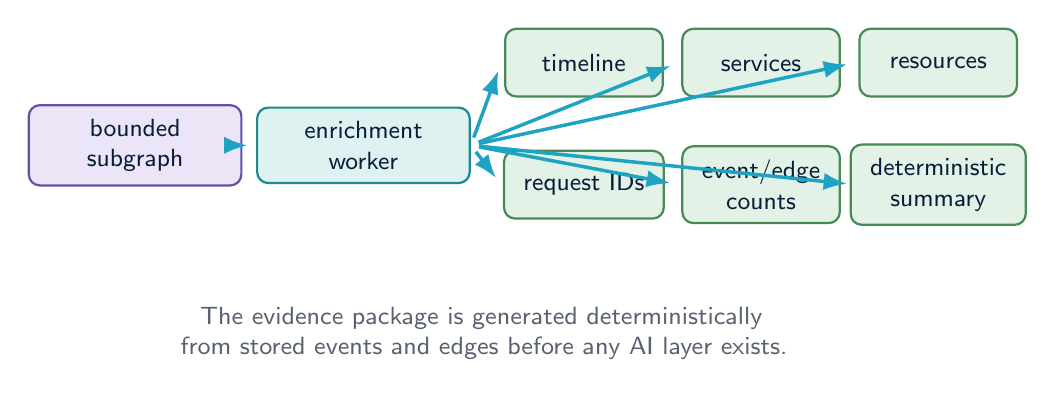
\begin{tikzpicture}[x=1cm,y=1cm]
  \node[graph,minimum width=2.7cm] (sub) at (1.6,3.05) {bounded\\subgraph};
  \node[transform,minimum width=2.7cm] (en) at (4.5,3.05) {enrichment\\worker};
  \node[ok,minimum width=2.0cm] at (7.3,4.1) {timeline};
  \node[ok,minimum width=2.0cm] at (9.55,4.1) {services};
  \node[ok,minimum width=2.0cm] at (11.8,4.1) {resources};
  \node[ok,minimum width=2.0cm] at (7.3,2.55) {request IDs};
  \node[ok,minimum width=2.0cm] at (9.55,2.55) {event/edge\\counts};
  \node[ok,minimum width=2.0cm] at (11.8,2.55) {deterministic\\summary};
  \draw[flow] (sub)--(en);
  \foreach \x/\y in {7.3/4.1,9.55/4.1,11.8/4.1,7.3/2.55,9.55/2.55,11.8/2.55}{\draw[flow] (en.east)--(\x-1.05,\y);}
  \node[note,text width=10.3cm] at (6,.66) {The evidence package is generated deterministically from stored events and edges before any AI layer exists.};
\end{tikzpicture}
\end{frame}

\begin{frame}{12. Horizon Investigation Workspace}
\progress{Teal}
\centering
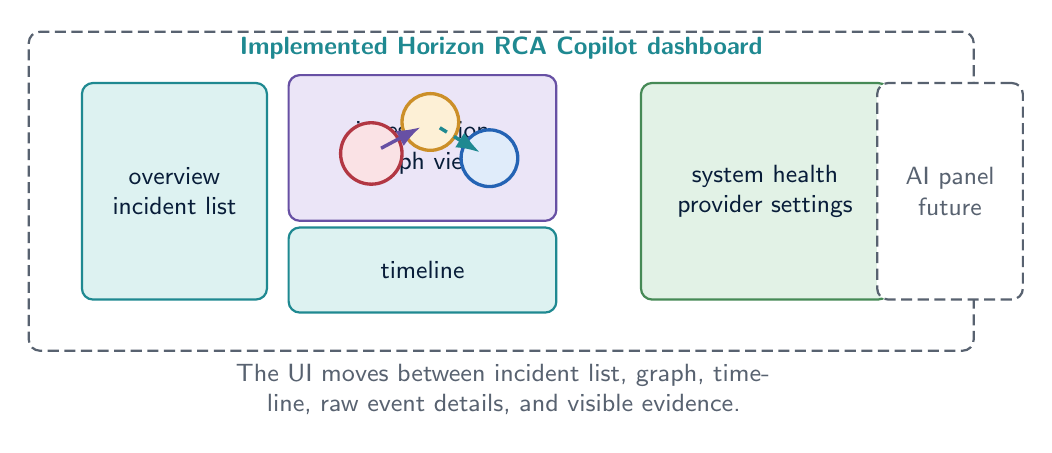
\begin{tikzpicture}[x=1cm,y=1cm]
  \node[future,minimum width=12.0cm,minimum height=4.05cm] at (6,3.0) {};
  \node[label,text=Teal] at (6,4.82) {Implemented Horizon RCA Copilot dashboard};
  \node[transform,minimum width=2.35cm,minimum height=2.75cm] at (1.85,3.0) {overview\\incident list};
  \node[graph,minimum width=3.4cm,minimum height=1.85cm] at (5.0,3.55) {investigation\\graph view};
  \node[transform,minimum width=3.4cm,minimum height=1.08cm] at (5.0,2.0) {timeline};
  \node[ok,minimum width=3.15cm,minimum height=2.75cm] at (9.35,3.0) {system health\\provider settings};
  \node[future,minimum width=1.85cm,minimum height=2.75cm] at (11.7,3.0) {AI panel\\future};
  \node[nodeErr] at (4.35,3.48) {};
  \node[nodeWarn] at (5.1,3.88) {};
  \node[nodeInfo] at (5.85,3.42) {};
  \draw[req] (4.35,3.48)--(5.1,3.88);
  \draw[res] (5.1,3.88)--(5.85,3.42);
  \node[note,text width=10.8cm] at (6,.48) {The UI moves between incident list, graph, timeline, raw event details, and visible evidence.};
\end{tikzpicture}
\end{frame}

\begin{frame}{13. Dynamic Graph Interaction Concept}
\progress{Teal}
\centering
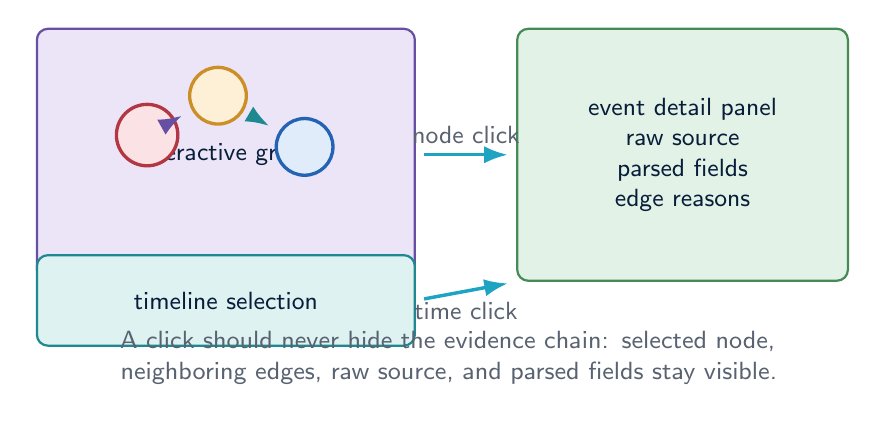
\begin{tikzpicture}[x=1cm,y=1cm]
  \node[graph,minimum width=4.8cm,minimum height=3.2cm] (graph) at (3.2,3.0) {interactive graph};
  \node[transform,minimum width=4.8cm,minimum height=1.15cm] (timeline) at (3.2,1.15) {timeline selection};
  \node[ok,minimum width=4.2cm,minimum height=3.2cm] (detail) at (9.0,3.0) {event detail panel\\raw source\\parsed fields\\edge reasons};
  \node[nodeErr] (n1) at (2.2,3.25) {};
  \node[nodeWarn] (n2) at (3.1,3.75) {};
  \node[nodeInfo] (n3) at (4.2,3.1) {};
  \draw[req] (n1)--(n2); \draw[res] (n2)--(n3);
  \draw[flow] (graph.east)--node[above,note]{node click}(detail.west);
  \draw[flow] (timeline.east)--node[below,note]{time click}(detail.south west);
  \node[note,text width=10.4cm] at (6,.42) {A click should never hide the evidence chain: selected node, neighboring edges, raw source, and parsed fields stay visible.};
\end{tikzpicture}
\end{frame}

\begin{frame}{14. Provider-Agnostic AI/RAG Future}
\progress{Green}
\centering
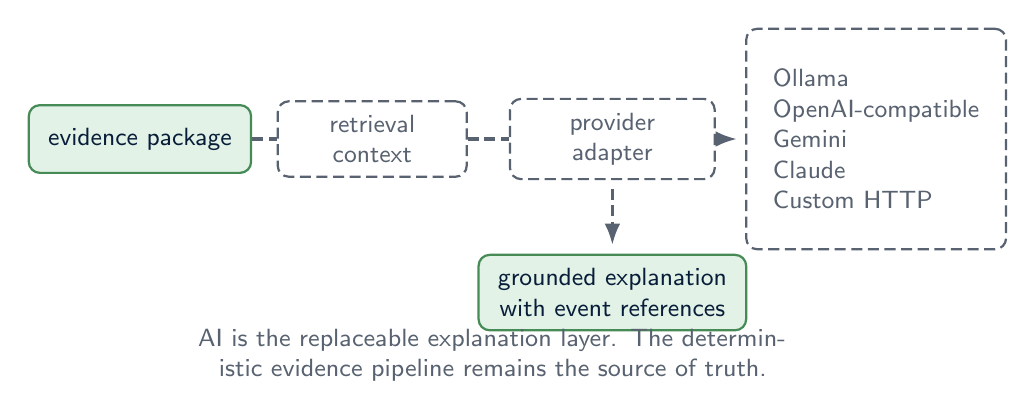
\begin{tikzpicture}[x=1cm,y=1cm]
  \node[ok,minimum width=2.8cm] (ev) at (1.55,3.2) {evidence package};
  \node[future,minimum width=2.4cm] (ctx) at (4.5,3.2) {retrieval\\context};
  \node[future,minimum width=2.6cm] (adapter) at (7.55,3.2) {provider\\adapter};
  \node[future,minimum width=3.3cm,minimum height=2.8cm,align=left] (providers) at (10.9,3.2) {
    Ollama\\OpenAI-compatible\\Gemini\\Claude\\Custom HTTP};
  \node[ok,minimum width=3.0cm] at (7.55,1.25) {grounded explanation\\with event references};
  \draw[futureline] (ev)--(ctx)--(adapter)--(providers);
  \draw[futureline] (adapter)--(7.55,1.75);
  \node[note,text width=10.8cm] at (6,.45) {AI is the replaceable explanation layer. The deterministic evidence pipeline remains the source of truth.};
\end{tikzpicture}
\end{frame}

\begin{frame}{15. OpenStack-Native Deployment}
\progress{Green}
\centering
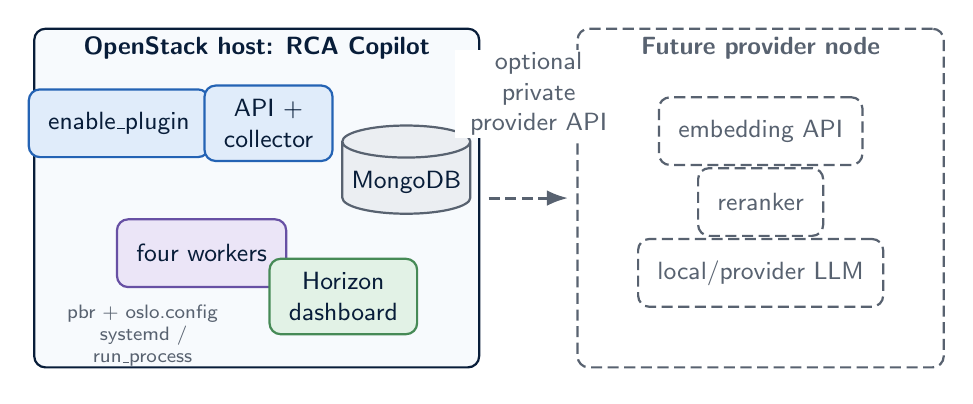
\begin{tikzpicture}[x=1cm,y=1cm]
  \node[box,draw=DeepNavy,fill=Canvas,minimum width=5.65cm,minimum height=4.3cm] (mac) at (3.3,2.8) {};
  \node[label] at (3.3,4.7) {OpenStack host: RCA Copilot};
  \node[service] at (1.55,3.75) {enable\_plugin};
  \node[service] at (3.45,3.75) {API +\\collector};
  \node[storage] at (5.2,3.0) {MongoDB};
  \node[graph] at (2.6,2.1) {four workers};
  \node[ok] at (4.4,1.55) {Horizon\\dashboard};
  \node[box,draw=Slate,dash pattern=on 4pt off 2pt,fill=white,minimum width=4.65cm,minimum height=4.3cm] (msi) at (9.7,2.8) {};
  \node[label,text=Slate] at (9.7,4.7) {Future provider node};
  \node[future] at (9.7,3.65) {embedding API};
  \node[future] at (9.7,2.75) {reranker};
  \node[future] at (9.7,1.85) {local/provider LLM};
  \draw[futureline] (mac.east)--(msi.west);
  \node[note,fill=white,inner sep=1pt,text width=2.05cm] at (6.88,4.12) {optional private\\provider API};
  \node[note,font=\scriptsize,text width=2.2cm] at (1.85,1.05) {pbr + oslo.config\\systemd / run\_process};
\end{tikzpicture}
\end{frame}

\begin{frame}{16. Final Full Architecture}
\progress{Green}
\centering
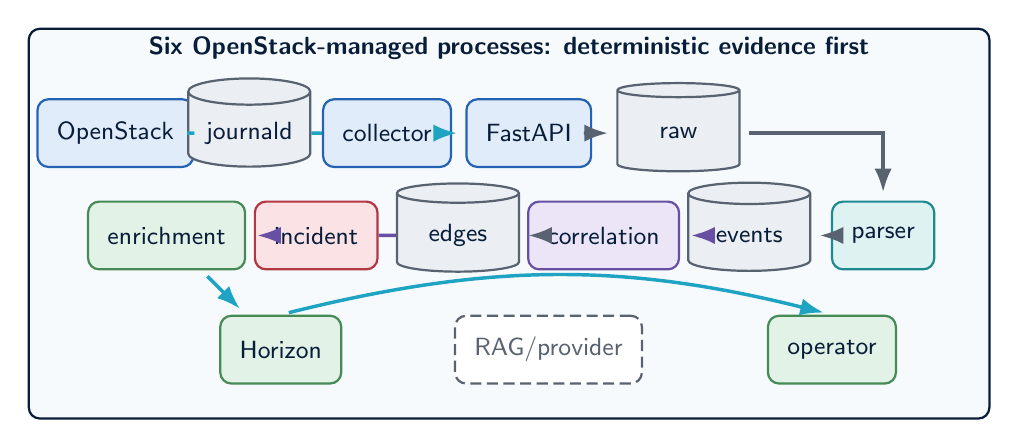
\begin{tikzpicture}[x=1cm,y=1cm]
  \node[box,draw=DeepNavy,fill=Canvas,minimum width=12.2cm,minimum height=4.95cm] at (6,2.85) {};
  \node[label] at (6,5.08) {Six OpenStack-managed processes: deterministic evidence first};
  \node[service] (os) at (1.0,4.0) {OpenStack};
  \node[storage] (j) at (2.7,4.0) {journald};
  \node[service] (col) at (4.45,4.0) {collector};
  \node[service] (api) at (6.25,4.0) {FastAPI};
  \node[storage] (raw) at (8.15,4.0) {raw};
  \node[transform] (parse) at (10.75,2.7) {parser};
  \node[storage] (parsed) at (9.05,2.7) {events};
  \node[graph] (corr) at (7.2,2.7) {correlation};
  \node[storage] (edges) at (5.35,2.7) {edges};
  \node[err] (inc) at (3.55,2.7) {incident};
  \node[ok] (en) at (1.65,2.7) {enrichment};
  \node[ok] (hor) at (3.1,1.25) {Horizon};
  \node[future] (rag) at (6.5,1.25) {RAG/provider};
  \node[ok] (op) at (10.1,1.25) {operator};
    \draw[flow] (os)--(j)--(col)--(api);
    \draw[data] (api)--(raw);
    \draw[data] (raw.east)-|(parse.north);
    \draw[data] (parse)--(parsed);
    \draw[req] (parsed)--(corr);
    \draw[data] (corr)--(edges);
    \draw[req] (edges)--(inc)--(en);
    \draw[flow] (en)--(hor);
    \draw[flow] (hor.north) to[bend left=14] (op.north);
\end{tikzpicture}
\end{frame}

\begin{frame}{17. Validation Plan}
\progress{Green}
\centering
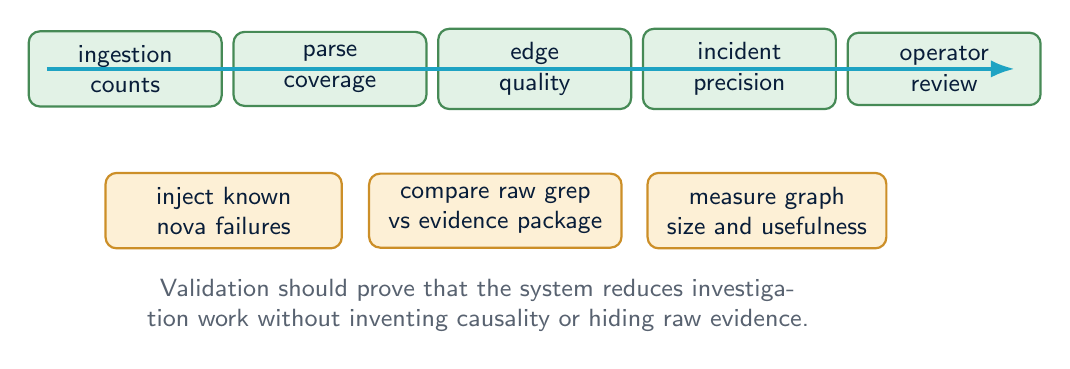
\begin{tikzpicture}[x=1cm,y=1cm]
  \node[ok,minimum width=2.45cm] at (1.55,3.55) {ingestion\\counts};
  \node[ok,minimum width=2.45cm] at (4.15,3.55) {parse\\coverage};
  \node[ok,minimum width=2.45cm] at (6.75,3.55) {edge\\quality};
  \node[ok,minimum width=2.45cm] at (9.35,3.55) {incident\\precision};
  \node[ok,minimum width=2.45cm] at (11.95,3.55) {operator\\review};
  \node[warn,minimum width=3.0cm] at (2.8,1.75) {inject known\\nova failures};
  \node[warn,minimum width=3.0cm] at (6.25,1.75) {compare raw grep\\vs evidence package};
  \node[warn,minimum width=3.0cm] at (9.7,1.75) {measure graph\\size and usefulness};
  \draw[flow] (.45,3.55)--(12.95,3.55);
  \node[note,text width=10.6cm] at (6,.55) {Validation should prove that the system reduces investigation work without inventing causality or hiding raw evidence.};
\end{tikzpicture}
\end{frame}

\begin{frame}{18. Roadmap and Final Takeaway}
\progress{Green}
\centering
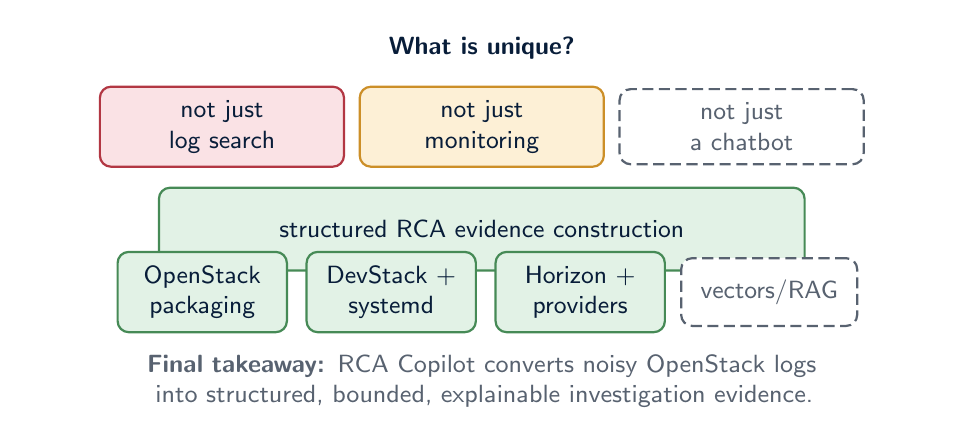
\begin{tikzpicture}[x=1cm,y=1cm]
  \node[label] at (6,4.55) {What is unique?};
  \node[err,minimum width=3.1cm] at (2.7,3.55) {not just\\log search};
  \node[warn,minimum width=3.1cm] at (6.0,3.55) {not just\\monitoring};
  \node[future,minimum width=3.1cm] at (9.3,3.55) {not just\\a chatbot};
  \node[ok,minimum width=8.2cm,minimum height=1.05cm] at (6,2.25) {structured RCA evidence construction};
  \node[ok,minimum width=2.15cm] at (2.45,1.45) {OpenStack\\packaging};
  \node[ok,minimum width=2.15cm] at (4.85,1.45) {DevStack +\\systemd};
  \node[ok,minimum width=2.15cm] at (7.25,1.45) {Horizon +\\providers};
  \node[future,minimum width=2.15cm] at (9.65,1.45) {vectors/RAG};
  \node[note,text width=11.3cm] at (6,.32) {\textbf{Final takeaway:} RCA Copilot converts noisy OpenStack logs into structured, bounded, explainable investigation evidence.};
\end{tikzpicture}
\end{frame}

\end{document}
